
\section{Xapian}

\subsection{Installation}

Der empfohlene Installationsweg für Xapian führt über die Paketquelle (PPA) der Entwickler. Nachdem dieses eingefügt wurde, kann Xapian entweder in einer C++ oder Python Variante installiert werden. 

Um die Suchmaschine auch über PHP anzusprechen ist es notwendig, den PHP-Connector aus Lizenzgründen selbst zu bauen. Dabei muss vorher ein Eintrag, der ausweist, dass aus dieser Quelle auch Source-Code geladen werden kann, in den Paketquellen hinzugefügt werden. Danach kann der Klient mithilfe von Make gebaut werden.

Allerdings ist der Server bisher nur lokal ansprechbar. Um dies zu ändern, muss ein TCP-Server für Xapian gestartet werden. Um diesen zu nutzen ist es vonnöten, ein weiteres Paket aus der Paketquelle zu installieren. Damit der Server gestartet werden kann, muss zuerst ein Index, der bei Xapian Database genannt wird, gebaut werden. Dazu mehr in dem Teil \ref{xap:index}. Danach kann der Server auf einen beliebigen Port gestartet werden.

\subsection{Indexierung}
\label{xap:index}

Durch die fehlende Dokumentation zur Indexierung von MySQL-Datenbanken, wurde erstmal ein Beispiel zum Import einer CSV-Datei durchgearbeitet. Darin war dann zu sehen, dass der komplette Datenimport manuell geschrieben werden musste. Auf dieser Basis wurde daraufhin ein eigener Importer für MySQL geschrieben \ref{lst:XapPhp}:

\begin{lstlisting}[language=php, frame=single, label={lst:XapPhp}, morekeywords={type,uninvertible,indexed,stored,field,multiValued, name}, caption=Skript zur Indexierung der Daten in Xapian,captionpos=b] 
<?php
require_once("xapian.php");

//Open MYSQL-Connection and Run Query. Save the Output in $result

// Create or open the database we're going to be writing to.
$db = new XapianWritableDatabase($xapianDb, Xapian::DB_CREATE_OR_OPEN);
// Set up a TermGenerator that we'll use in indexing.
$termgenerator = new XapianTermGenerator();
$termgenerator->set_stemmer(new XapianStem('de')); //Setup Stemmer

while ($row = $result->fetch_assoc()) { //Loop through MySQL-Rows

	$identifier = $row['id'];
	unset($row['id']);
	// Create new Row for the starting Letter
	$searchIndexLetter = $row['original_bezeichnung'][0];

	$doc = new XapianDocument(); // Create new Document
	$termgenerator->set_document($doc); //Put it into the Term-Generator

	// Index the field with a suitable prefix.
	$termgenerator->index_text($searchIndexLetter, 1, 'K'); 
	// Make it available for Search
	$termgenerator->index_text($searchIndexLetter); 

	foreach ($row as $index) {
		if ($index = '') { //Xapian cant Index Empty Fields
			$index = 'EMPTY';
		}
		$termgenerator->increase_termpos(); // Make Space between Entries
		$termgenerator->index_text($index); // Add Every Field
	}
	$doc->set_data(json_encode($row)); // Store all the fields

	$idterm = "Q".$identifier; //Set ID to not have Duplicates
	$doc->add_boolean_term($idterm);
	$db->replace_document($idterm, $doc);
}
$conn->close();
\end{lstlisting}

In Zeile 10 wird ein Stemmer verwendet, welcher dazu dient, wenn zum Beispiel der Plural eines Wortes gesucht wird, auch den Singular zu finden.

In Zeile 23 wird ein Feld mit einem Präfix indexiert. Dies dient dazu, diese Zeile für die spätere Suche auszuweisen. Die Präfixe werden dabei vor die Zeile geschrieben und bei der Suche wieder herausgefiltert. 

Die anderen Felder wurden für die generelle Suche ohne Präfix indexiert. Zuletzt noch der Grund, warum leere Zeichenketten gegen das Wort 'EMPTY' ausgetauscht werden. Dies beruht darauf, dass Xapian es nicht erlaubt, leere Zeichenketten zu indexieren.

Als nun das PHP-Script auf dem Server gestartet wurde, musste noch eine Warnung behoben werden. Dazu wurde die php.ini angepasst, indem der Eintrag 'enable\_dl' gemacht wurde. Damit können jetzt Erweiterungen auch zur Laufzeit geladen werden, was die Bibliothek von Xapian benötigt.

Die Indexierung lief dabei äußerst schnell in unter einer Minute ab.

\subsection{Oberfläche}

Xapian besitzt keine Oberfläche zur Verwaltung. Allerdings kann sich ein Such-Frontend installiert werden, welches allerdings hier nicht geprüft wurde, da die Dokumentation noch nicht verfügbar war.

\subsection{Dokumentation}

Bei dem letzten Versionsupgrade wurde die Dokumentation von Xapian komplett umgeschrieben. Diese neue Dokumentation hat bisher noch viele Lücken und Todo-Boxen \ref{img:xapianDoku}.

Zu der Installation von dem TCP-Server war auch nichts in der neuen Dokumentation zu finden. Beim Durchsuchen des Internets, wie der Server extern ansprechbar gemacht werden kann, konnte eine Seite der alten Dokumentation gefunden werden, welche den Befehl zum Starten vermerkt hatte. Nachdem dieser Befehl ausgeführt wurde, wurde gemeldet, dass für diesen Befehl ein weiteres Paket installiert werden musste. Dieses Paket wurde in der Dokumentation nicht vermerkt. 

Generell bietet die Dokumentation, in der aktuellen Form, nur einen sehr grundlegenden Einblick in das System. Positiv anzumerken ist allerdings, dass Xapian ein Beispiel zu Indexierung von Daten mit Code in allen verfügbaren Programmiersprachen auf Github bereitstellt. In der Dokumentation wird allerdings nur das Python-Beispiel eingegangen.

\begin{figure}
	\centering
	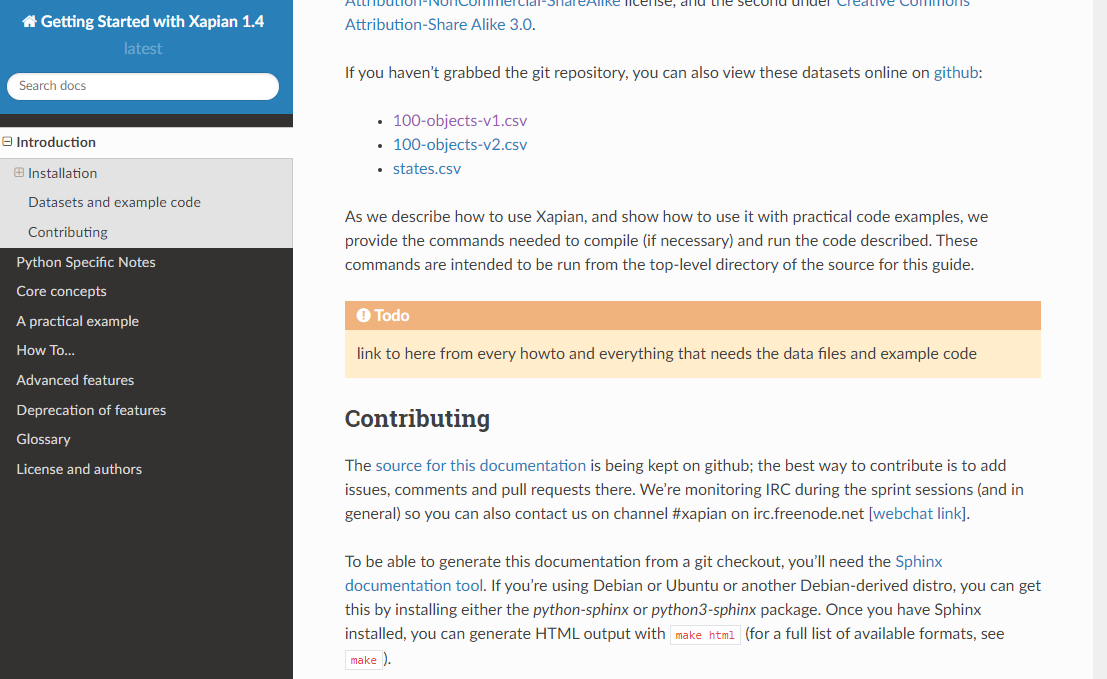
\includegraphics[width=1\linewidth]{images/xapian_doku.png}
	\caption{Screenshot von der Xapian Dokumentation}
	\label{img:xapianDoku}
\end{figure}

\subsection{Absetzen einer Anfrage und Integration in PHP}

Xapian besitzt keine REST-Schnittstelle. Daher wird der Befehl direkt auf mit PHP-Aufrufen gesendet. Dabei konnte aufgrund des Zeitkon­tin­gents die Remote Ausführung nicht getestet werden, da der Aufwand die PHP-Erweiterung auf Windows zu bauen, zu hoch war. Die Datei wurde deshalb direkt auf den Server ausgeführt, was bei der Laufzeit bedacht werden muss. 

Der Grund, warum eine eigene Zeile für den Buchstaben ausgewiesen werden muss, ist, dass Xapian generell nur Volltext ausweist. Es wurde zuerst versucht, mit Wildcards zu arbeiten, allerdings ergaben sich dabei dieselben Probleme, wie bei den anderen Suchmaschinen.

\begin{lstlisting}[language=php, frame=single, label={lst:XapPhpQuery}, 
	morekeywords={type,uninvertible,indexed,stored,field,multiValued, name}, caption=Skript zur Suche von Daten in Xapian,captionpos=b] 
// Require xapian.php and declare variables

$db = new XapianDatabase('db'); //Open Database

$queryParser = new XapianQueryParser();
//Set Prefix for Search
$queryParser->add_prefix("searchIndexLetter", "K"); 
$query = $queryParser->parse_query('S'); // Parse Query

//Loop for and time Results
// Use an Enquire object on the database to run the query
$enquire = new XapianEnquire($db);
$enquire->set_query($query);
$matches = $enquire->get_mset(0, 2147483647)->begin();
foreach ($matches as $pointer){
	$doc = $matches->get_document()->get_data();
	//$fields = json_decode($doc);
	$count++;
}
// Output Time for Run
//End Loop 
// Output Median Time
	
\end{lstlisting}

Nachdem die Abfrage die ersten hundert Male durchgelaufen war, war die Zeit mit 0.0044 Sekunden im Durchschnitt für die Ergebnisse sehr gering. Dies liegt daran, dass die Ergebnisse erstmal nur Pointer auf die kompletten Daten sind. 

Um nun alle Daten zu erhalten, muss nochmals ein gesonderter Befehl geschickt werden. Deswegen ist im Code ab Zeile 15 auch eine For-Schleife, welche die Datensätze für alle Pointer holt. Foreach verschiebt dabei automatisch den Pointer von den Ergebnissen. Wichtig ist, dass der Count ein Programmschritt ist, der theoretisch die Laufzeit erhöht und nicht für die normale Abfrage genutzt werden würde. Allerdings wurde diese Erhöhung hingenommen, um festzustellen, ob immer alle Ergebnisse korrekt geliefert werden.
Die auskommentierte Zeile würde das Objekt nun als Array mit Indices zurückgeben. 

Die Abfrage für das Abholen der Daten dauerte nun im Durchschnitt 0.22 Sekunden, was immer noch sehr schnell ist. Allerdings muss dabei bedacht werden, dass die Abfrage direkt auf dem Server lief, wodurch es keine Latenzzeit gab.
